\documentclass[11pt, openright]{book}

    % Cover Variables
    \newcommand{\ctoptitle}{}
    \newcommand{\ctitle}{Mini-Projet}
    \newcommand{\cautor}{Lucas Lescure - Tom Paillet}
    \newcommand{\cdate}{28.04.2024}
    \newcommand{\sectittle}{Lettris - Tetris avec des lettres}


    % Header Variables
        \newcommand{\headRE}{Mini-Projet - Lettris}
        \newcommand{\headLE}{\emph{\rightmark}}
        \newcommand{\footRE}{L.Lescure T.Paillet$-$ \cdate}
        \newcommand{\footLE}{\emph{\thepage}}

    % TOC Variables
        \newcommand{\toctitle}{Table des contenus}
        
        \newcommand{\tocchapter}{Chapter}
        \newcommand{\toccount}{3}
  
    % Chapter Variables
        \newcommand{\chvar}{Chapter -}

\usepackage[a4paper, total={16cm, 22.125cm}]{geometry}

% Page Style
\usepackage[]{environ}
% Cover Page 
\usepackage{tikz}
\makeatletter
\def\parsecomma#1,#2\endparsecomma{\def\page@x{#1}\def\page@y{#2}}
\tikzdeclarecoordinatesystem{page}{
    \parsecomma#1\endparsecomma
    \pgfpointanchor{current page}{north east}
    % Save the upper right corner
    \pgf@xc=\pgf@x%
    \pgf@yc=\pgf@y%
    % save the lower left corner
    \pgfpointanchor{current page}{south west}
    \pgf@xb=\pgf@x%
    \pgf@yb=\pgf@y%
    % Transform to the correct placement
    \pgfmathparse{(\pgf@xc-\pgf@xb)/2.*\page@x+(\pgf@xc+\pgf@xb)/2.}
    \expandafter\pgf@x\expandafter=\pgfmathresult pt
    \pgfmathparse{(\pgf@yc-\pgf@yb)/2.*\page@y+(\pgf@yc+\pgf@yb)/2.}
    \expandafter\pgf@y\expandafter=\pgfmathresult pt
}
\makeatother


% Object formatting
\usepackage[12pt]{moresize}
\usepackage[]{anyfontsize}
\usepackage{titlesec}
\usepackage{import}
\usepackage{floatrow}
\usepackage{enumitem}
\usepackage{changepage}
\usepackage[normalem]{ulem}
\usepackage{array}
\newcommand{\ul}[1]{\underline{#1}}

\usepackage[]{chngcntr}
\usepackage{ifthen}
\ifthenelse{\figcountdepth > 1}
  {\counterwithin{figure}{section}\counterwithin{table}{section}}
  {}

\usepackage[format=plain, labelfont=it, textfont=it]{caption}
\makeatletter
\def\@makecaption#1#2{%
    \vskip\abovecaptionskip
    \sbox\@tempboxa{\textit{#1.} #2}

       
   

    \ifdim \wd\@tempboxa >\hsize
        #1. #2\par
    \else
        \global \@minipagefalse
        \hb@xt@\hsize{\hfil\box\@tempboxa\hfil}
    \fi
    \vskip\belowcaptionskip}
\makeatother

\DeclareCaptionFormat{underline}{\uline{#1#2#3}\par}

% Sections
\titleformat{\section}{\fontsize{16}{19.2}\bfseries}{\thesection.}{0.25em}{}
\titleformat{\subsection}{\fontsize{14}{16.8}\bfseries}{\tab\thesubsection.}{0.25em}{}
\titleformat{\subsubsection}{\fontsize{10}{12}}{\uline{\thesubsubsection)\enspace}}{0em}{\uline}





% Geometry

% Typewritting

\setlength{\parskip}{1em}
\setlength{\parindent}{0em}


\newenvironment{items}[3][0pt]
{\def\closesep{#3}
    \vspace{#2}
    \begin{itemize}
        \setlength{\itemsep}{#1}
        \setlength{\topsep}{0pt}
        \setlength{\partopsep}{0pt}}
        {\end{itemize}
    \vspace{\closesep}}

\newenvironment{enum}[3][0pt]
{\defclosesep{#3}
    \vspace{#2}
    \begin{enumerate}
        \setlength{\itemsep}{#1}
        \setlength{\topsep}{0pt}
        \setlength{\partopsep}{0pt}}
        {\end{enumerate}
    \vspace{\closesep}}

\newenvironment{eq}[2]
{\def\closesep{#2}
    \vspace{#1}
    \begin{align*}}
        {\end{align*}
    \vspace{\closesep}}

\newenvironment{lfeq}[2]
{\def\closesep{#2}
    \vspace{#1}
    \begin{flalign*}}
        {\end{flalign*}
    \vspace{\closesep}}
% List Formatting


\NewEnviron{dent}[1]{
    \vspace{-10pt}
    \begin{adjustwidth}{7mm}{}
        \uline{#1}\hspace{2mm}
        \BODY
    \end{adjustwidth}
    \vspace{-10pt}
}


\usepackage[framemethod=tikz]{mdframed}
\newcounter{count_theorem}[section]\setcounter{count_theorem}{0}
\newcommand{\thetheorem}{\arabic{count_theorem}}

\newcounter{count_exercise}[section]\setcounter{count_exercise}{0}
\newcommand{\theexercise}{\arabic{count_exercise}}


\newenvironment{theorem}[1][]{
    \refstepcounter{count_theorem}
    \mdfsetup{
        linecolor=red!30,
        innerbottommargin=10pt,
        linewidth=2pt,
        topline=false,
        bottomline=false,
        rightline=false,
        shadow=true,
        shadowsize=4.5pt,
        frametitlerule=false,
        apptotikzsetting={
                \tikzset{
                    mdfbackground/.append style={
                            left color=red!8,right color=red!3
                        }
                }
            }
    }
    \begin{mdframed}[]\relax
        \ifstrempty{#1}
        {\textbf{Theorem~\thetheorem.} }
        {\textbf{Theorem~\thetheorem.~#1} }
        }
        {\end{mdframed}\vspace{-10pt}
}

\newenvironment{note}{
    \mdfsetup{innertopmargin=5pt,
        linecolor=gray!30,
        linewidth=2pt,
        topline=false,
        bottomline=false,
        rightline=false,
        frametitleaboveskip=0pt,
        shadow=false,
        shadowsize=4pt,
        frametitlerule=false,
        apptotikzsetting={
                \tikzset{
                    mdfbackground/.append style={
                            left color=gray!8,right color=gray!3
                        }
                }
            }
    }
    \begin{mdframed}[]\relax
        \textbf{Note. }
        }
        {\end{mdframed}\vspace{-10pt}
}

\newenvironment{example}{
    \mdfsetup{innertopmargin=5pt,
        linecolor=green!30,
        linewidth=2pt,
        topline=false,
        bottomline=false,
        rightline=false,
        frametitleaboveskip=0pt,
        shadow=false,
        shadowsize=4pt,
        frametitlerule=false,
        apptotikzsetting={
                \tikzset{
                    mdfbackground/.append style={
                            left color=green!7,right color=green!2
                        },
                    mdfframetitlebackground/.append style={
                            left color=green!7,right color=green!2
                        }
                }
            }
    }
    \begin{mdframed}[]\relax
        \textbf{Example. }
        }
        {\end{mdframed}\vspace{-10pt}
}


\usetikzlibrary{calc,arrows}

\tikzset{
    excursus arrow/.style={%
            line width=2pt,
            draw=gray!40,
            rounded corners=2ex,
        },
    excursus head/.style={
            fill=white,
            font=\bfseries\sffamily,
            text=gray!80,
            anchor=base west,
        },
    excursus line/.style={%
            line width=2pt,
            draw=gray!40,
            rounded corners=2ex,
        }
}

\newenvironment{exercise}[1][]{%
    \refstepcounter{count_exercise}
    \mdfsetup{
        singleextra={
                \path let \p1=(P), \p2=(O) in (\x2,\y1) coordinate (Q);
                \path let \p1=(Q), \p2=(O) in (\x1,{(\y1-\y2)/2}) coordinate (M);
                \path [excursus line] ($(O)+(5em,0ex)$) -| (M) |- ($(Q)+(20em,0ex)$);
                \node [excursus head] at ($(Q)+(2.5em,-0.75pt)$) {\ifstrempty{#1}{Exercise \theexercise}{Exercise \theexercise:~#1}};},
        firstextra={
                \path let \p1=(P), \p2=(O) in (\x2,\y1) coordinate (Q);
                \path [excursus arrow,-to] (O) |- ($(Q)+(12em,0ex)$) .. controls +(0:16em) and +(185:6em) .. ++(23em,2ex);},
        middlelinewidth=2.5em,middlelinecolor=white,
        hidealllines=true,topline=true,
        innertopmargin=0.5ex,
        innerbottommargin=2.5ex,
        innerrightmargin=2pt,
        innerleftmargin=2ex,
        skipabove=0.87\baselineskip,
        skipbelow=0.62\baselineskip,
    }
    \begin{mdframed}[]\relax}
        {\end{mdframed}\vspace{-10pt}
}

% Functions and Data Plotting
\usepackage{subfig,wrapfig,adjustbox,multirow}


% Plotting Style
\usepackage{graphicx,pgfplots}
\usetikzlibrary{arrows}
\usetikzlibrary {patterns,patterns.meta}
\usepgfplotslibrary{fillbetween}
\pgfplotsset{compat=1.18}

\usepgfplotslibrary{units}
% Logarithmic Scale
\pgfplotsset{
    log x ticks with fixed point/.style={
            xticklabel={
                    \pgfkeys{/pgf/fpu=true}
                    \pgfmathparse{exp(\tick)}%
                    \pgfmathprintnumber[fixed relative, precision=3]{\pgfmathresult}
                    \pgfkeys{/pgf/fpu=false}
                }
        }
}


% Mathematics

% Formatting
\usepackage{amsmath}
\usepackage{esvect}
\usepackage{amsfonts}
\usepackage{tasks,environ}
\usepackage{xargs}
\usepackage{esint}
\usepackage[]{listings}


\usepackage[english]{babel}
\usepackage{amsthm}
%\newtheorem{theorem}{Theorem}
%\newtheorem{proof}{Proof}



%Custom Shortcuts
\newcommand{\eqi}{\Leftrightarrow}
\newcommand{\lr}[1]{\left( #1 \right)}
\newcommand{\limit}[1]{\displaystyle{\lim_{#1}}}
\newcommand{\tab}{\hspace*{7mm}}
\newcommand{\ds}[1]{\displaystyle{#1}}
\newcommand{\floor}[1]{\lfloor #1 \rfloor}
\newcommand{\R}{\mathbb{R}}
\newcommand{\N}{\mathbb{N}}
\newcommand{\Z}{\mathbb{Z}}
\newcommand{\C}{\mathbb{C}}
\newcommand{\K}{\mathbb{K}}
\newcommand{\F}{\mathcal{F}}
\newcommand{\M}{\mathcal{M}}
\renewcommand{\l}{\lambda}
\newcommand{\seg}[1]{\overline{\rm {#1}}}
\newcommand{\Int}{\int\limits}
\newcommand{\ex}{\tab \uline{Example :}\hspace{0.2cm} }
\newcommand{\vard}{\partial}
\newcommand{\Q}{\mathcal{Q}}
\newcommand{\Vect}{\operatorname{Vect}}
\newcommand{\rg}{\operatorname{rg}}
\renewcommand{\dim}{\operatorname{dim}}
\renewcommand{\Re}{\operatorname{Re}}
\renewcommand{\Im}{\operatorname{Im}}
\renewcommand{\P}{\mathcal{P}}
\newcommand{\blr}[1]{\left\{#1\right\}}
\newcommand{\linecenter}[1]{\par\vspace{2mm} \centerline{#1}\par\vspace{-2mm}}
\newcommand{\dd}{\textrm{d}}
\newcommand{\supp}{\operatorname{Supp}}
\renewcommand{\vec}{\overrightarrow}
\renewcommand{\epsilon}{\varepsilon}

% Matrix Configurations

\makeatletter
\renewcommand*\env@matrix[1][*\c@MaxMatrixCols c]{%
    \hskip -\arraycolsep
    \let\@ifnextchar\new@ifnextchar
    \array{#1}}
\makeatother


% Colors
\usepackage{xcolor}
\newcommand{\blu}{\color{blue}}
\newcommand{\Red}{\color{red}}
\newcommand{\blac}{\color{black}}

\newcommand{\red}[1]{\textcolor{red}{#1}}

\usepackage{xcolor,xspace}
\usepackage{breqn}


% Headings  
\usepackage[Glenn]{fncychap}
\ChNumVar{\fontsize{40}{42}}
\ChTitleVar{\Large\sc}
\ChNameVar{\Large\sc}
\setlength\headheight{14.5pt}
\renewcommand\FmN[1]{\chvar}



\usepackage{fancyhdr}
\usepackage{ragged2e}

% Header & Footers
\renewcommand{\chaptermark}[1]{\markboth{#1}{#1}}
\renewcommand{\sectionmark}[1]{
    \markright{ #1}
}
\pagestyle{fancy}
\fancyhf{}
\fancyhead[LE,RO]{\headLE}
\fancyhead[RE,LO]{\headRE}
\fancyfoot[LE,RO]{\footLE}
\fancyfoot[RE,LO]{\footRE}
\renewcommand{\headrulewidth}{0.5pt}
\fancyheadoffset{1cm}

\fancypagestyle{plain}{%
    \fancyhf{} % clear all header and footer fields
    \fancyfoot[LE, RO]{\footLE}
    \renewcommand{\headrulewidth}{0pt}
    \renewcommand{\footrulewidth}{0pt}}


\fancypagestyle{nohead}{%
    \fancyhf{} % clear all header 
    \fancyfoot[LE, RO]{\footLE}
    \fancyfoot[LO, RE]{\footRE}}

    \fancypagestyle{head}{%
    \fancyhf{} % clear all header 
    \fancyhead[LE,RO]{\headLE}
\fancyhead[RE,LO]{\headRE}
\renewcommand{\headrulewidth}{0.5pt}
\fancyheadoffset{1cm}
    }


\fancypagestyle{bib}{%
    \fancyhf{} % clear all header and footer fields
    \fancyhead[CE, CO]{}
    \fancyfoot[LE, RO]{\footLE}
    \fancyfoot[LO, RE]{Bibliographie}}

% Table of Contents

\renewcommand*\thechapter{\arabic{chapter}} %Usually Roman
\renewcommand*\thesection{\arabic{section}}
\renewcommand*\thesubsubsection{\thesubsection.\alph{subsubsection}}
\makeatletter
\@removefromreset{section}{chapter}
\makeatother


% Table of Contents

\usepackage{titletoc}
\usepackage{ erewhon,cabin}
\usepackage[linktoc=all]{hyperref}
\renewcommand*\contentsname{\centerline{\toctitle}}

\setcounter{secnumdepth}{3}
\setcounter{tocdepth}{\toccount}

\usepackage[subfigure]{tocloft}
\setlength\cftparskip{0pt}

\usepackage{etoolbox}
\makeatletter
\pretocmd{\chapter}{\addtocontents{toc}{\protect\addvspace{5\p@}}}{}{}
\pretocmd{\section}{\addtocontents{toc}{\protect\addvspace{-10\p@}}}{}{}
\pretocmd{\subsection}{\addtocontents{toc}{\protect\addvspace{1\p@}}}{}{}
\makeatother


% Chapter Style
\titlecontents{chapter}
[11em]
{\bigskip}
{\bfseries\textsc\tocchapter~\textsc\thecontentslabel : \textsc}
{\hspace*{-5.5em}\textbf}
{\titlerule*[1pc]{ }}[\smallskip]

% Section Style
\titlecontents{section}
[0em] % i
{\bigskip\bfseries}
{\fontsize{11}{13.2}\bfseries\uline{\thecontentslabel.\enspace}\uline}
{\hspace*{-4em}\textbf}
{\hspace{0.5pt}\uline{\hspace*{\fill}}\contentspage}

% Subsection Style
\titlecontents{subsection}
[2em] % i
{\smallskip\bfseries}
{\fontsize{10}{12}\bfseries\thecontentslabel.\enspace}
{\hspace*{-4em}}
{\titlerule*[0.5pc]{.}\contentspage}

% Subsubsection Style
\titlecontents{subsubsection}
[4em] % i
{\smallskip}
{\fontsize{10}{12}\thecontentslabel)\enspace}
{\hspace*{-4em}}
{\titlerule*[0.5pc]{.}\contentspage}










    % figure support
    \usepackage{import}
    \usepackage{xifthen}
    \pdfminorversion=7
    \usepackage{pdfpages}
    \usepackage{transparent}
    \newcommand{\incfig}[1]{%
            \def\svgwidth{\columnwidth}
            \import{./figures/}{#1.pdf_tex}
    }

    \pdfsuppresswarningpagegroup=1


\begin{document}
% Spacing
% Section Spacing
\titlespacing\section{0pt}{3pt plus 2pt minus 2pt}{6pt plus 2pt minus 1pt}
\titlespacing\subsection{0pt}{0pt plus 1pt minus 1pt}{0pt plus 3pt minus 1pt}
\titlespacing\subsubsection{0pt}{0pt plus 0pt minus 0pt}{0pt plus 2pt minus 0pt}

\usetikzlibrary{shadows}

\newgeometry{left=2.5cm, width=16cm, bottom=2.5cm, top=2.5cm}






% Cover
% Cover
\definecolor{ccolor1}{RGB}{236,145,143}
\definecolor{ccolor2}{RGB}{131,168,192}
\definecolor{ccolor3}{RGB}{182,227,150}
\definecolor{ccolor4}{RGB}{171,206,145}

\usetikzlibrary{fadings}

\begin{titlepage}
    \newgeometry{top=1cm, width=21cm, bottom=1cm}

    \begin{tikzpicture}[remember picture,overlay,every node/.style={anchor=center}]

        \coordinate (Center) at (page cs: 0,-0.5);
        %F4E Logo
        \begin{scope}[scale = 1.5]
            \foreach \angle in {0,30,...,330} {
                    \filldraw[orange!50!yellow,line width=0.01pt,shift=(Center)] (\angle:3.8637) -- (\angle+30:3.8637) -- (0,0) -- (\angle:3.8637);
                    \draw[white, line width = 7pt,shift=(Center)] (\angle:2cm) arc (\angle-60:\angle:2cm);
                    \draw[white, line width = 7pt,shift=(Center)] (\angle+30:2cm) arc (\angle+90:\angle+30:2cm);
                }
            % Outer delimiter
            \foreach \angle in {15,45,...,345} {
                    \filldraw[white, line width = 7pt,shift=(Center)] (\angle:3.8637cm) arc (\angle-15:\angle+45:2cm) arc (\angle+15:\angle-15:2cm) arc (\angle+45:\angle+15:2cm);
                }
            % Inner delimiter
            \foreach \angle in {15,45,...,345} {
                    \filldraw[white, line width = 7pt,shift=(Center)] (\angle:1.0353cm) arc (\angle-75:\angle-45:2cm) arc (\angle+75:\angle+105:2cm) -- (0,0) -- (\angle:1.0353cm);
                }
            % Stars
            \foreach \angle in {0,30,...,330} {
                    \fill[orange!50!yellow,shift=(Center)] (\angle:1.03527cm) -- ++ (231:0.175) -- ++ (33:0.35) -- ++ (177:0.35) -- ++ (321:0.35) -- ++ (105:0.35) -- ++ (249:0.35) -- ++ (33:0.35);
                }
        \end{scope}

        \node[opacity =0.07, inner sep=0pt, anchor=east] at (current page.east){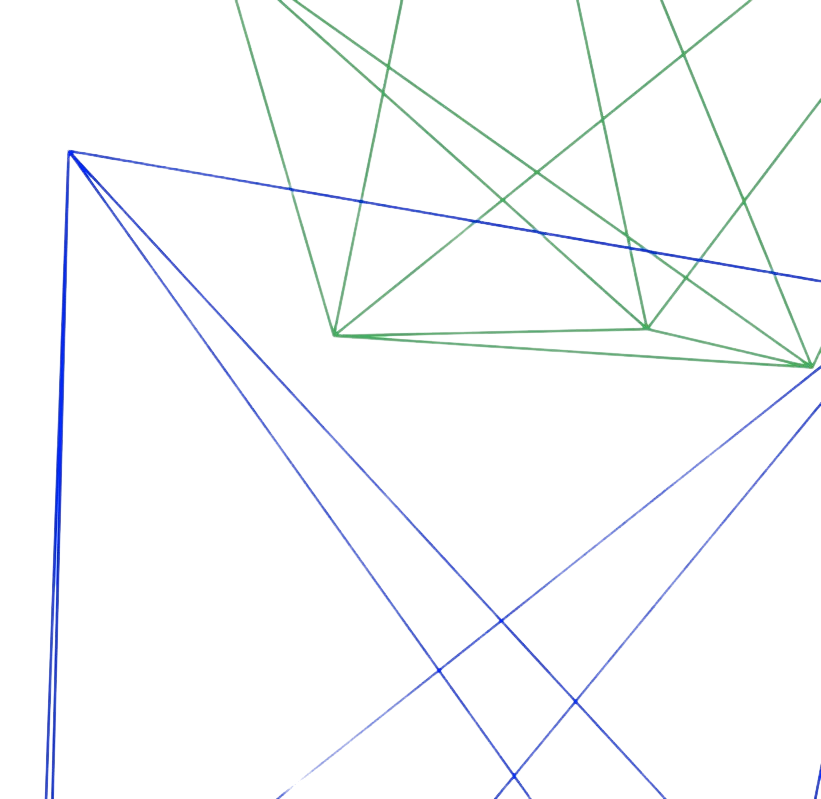
\includegraphics[width=0.5\paperwidth,height=\paperheight]{/root/.config/latex-utils/logos/invert1.png}};

        \node[opacity=0.07,inner sep=0pt, anchor=north west] at (current page.north west){
\includegraphics[width=0.5\paperwidth,height=0.5\paperheight]{/root/.config/latex-utils/logos/invert3.png}};




        \node at (page cs:0,0.345) {\Large\textsc{High School Observation and Learning Internship}};
        \node at (page cs:0,0.875) {\Large\bfseries\textsc{Observation Internship}};
        \node at (page cs:0,0.925) {\LARGE\bfseries\textsc{Lycée Français de Barcelone}};

        \node at (page cs:0.5,0) {\Large\textsc{Cyril Lescure - Pedagogical Tutor}};








        %\node[opacity=0.15, inner sep=0pt, anchor=south west] at (current page.south west){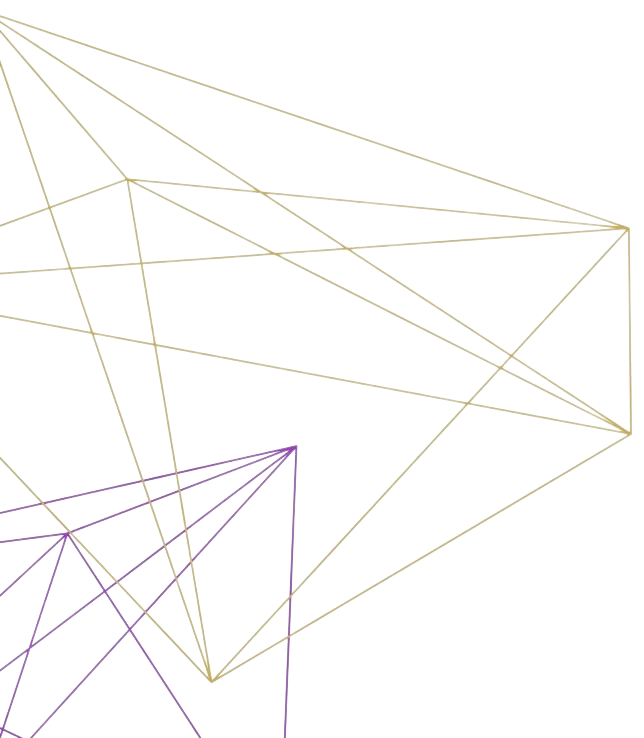
\includegraphics[width=0.5\paperwidth,height=0.5\paperheight]{/root/.config/latex-utils/logos/invert2.png}};

        \node at (page cs:0,0.5) {\fontsize{28}{28.8}\textbf{\ctoptitle}};
        \node at (page cs:0,0.425) {\fontsize{28}{28.8}\textbf{\ctitle}};
        \draw (page cs:0.5,0.375) -- (page cs:-0.5,0.375);
        \node at (page cs:0,0.245) {\LARGE\textsc{\cautor}};
        \node at (page cs:0,0.310) {\Large\textsc{03.06.2019 - 07.06.2019}};


    \end{tikzpicture}
\end{titlepage}


\newgeometry{width=18.625cm, bottom=2cm, top=2cm}

\tikz[remember picture, overlay] \node[opacity=0.3,inner sep=0pt, anchor=north east] at (current page.north east){
\includegraphics[angle=-90,origin=c,width=0.5\paperheight,height=0.5\paperwidth]{/root/.config/latex-utils/logos/invert3.png}};
\tikz[remember picture,overlay] \node[opacity=0.3,inner sep=0pt, anchor=south east] at (current page.south east){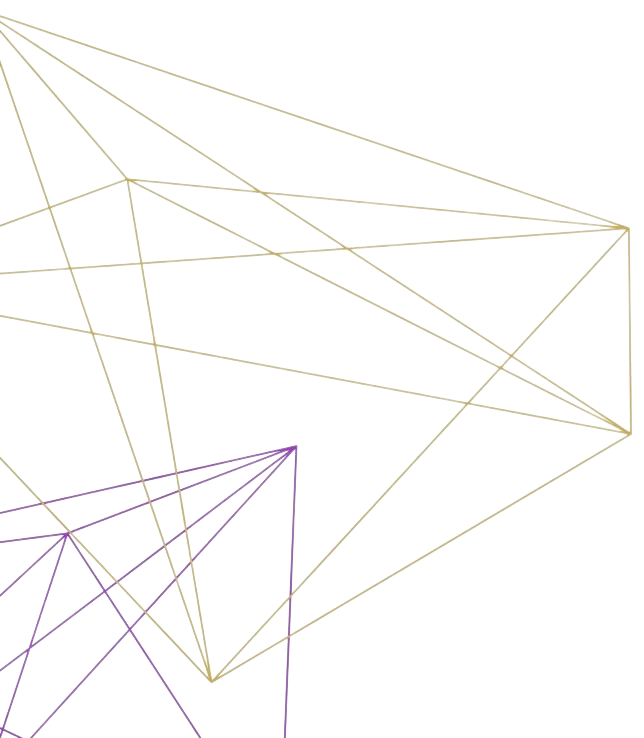
\includegraphics[angle=90,width=0.5\paperwidth,height=0.5\paperheight]{/root/.config/latex-utils/logos/invert2.png}};

\tableofcontents




    
    \newpage

    
     \section{Specification du jeu}

        \subsection{Principe}

            Le jeu Lettris est un jeu de type Tetris, c'est-à-dire que des blocs tombent du haut de l'écran et le joueur doit les placer de manière à former des lignes complètes pour les faire disparaître. La particularité de Lettris est que les blocs sont des lettres de l'alphabet et que le joueur doit former des mots pour les faire disparaître.

            Le jeu se déroule sur une grille de 10x15 cases et le joueur peut déplacer les blocs à gauche, droite, ou bien les faire tomber plus rapidement. Apres avoir formé un mot de plus de 4 lettres, les lettres disparaissent et le joueur gagne des points en fonction de la taille du mot. Le jeu se termine lorsqu'il n'est plus possible de rajouter des lettres à la grille. 
            
         \subsection{Fonctionnalités}
            En accord avec le cahier des charges, lorsque le jouer forme un mot, ceci incrémentera un compteur qui sera affiché dans la colonnes des mots formés. Pour ajouter sur ceci, le joueur aura a sa disposition un journal contenant les 10 derniers mots formés ainsi que les points gagnés par mots. Ces mots sont sauvegardés au fur et à mesure dans un fichier texte placé à  \texttt{./resources/foundWords.txt}. 

            De plus pour encourager un air compétitif, le joueur pourra consulter pendant que le jeu se déroule l'état de son score ainsi que le score maximal enregistré sur le jeu. L'historique des scores est sauvegardé à chaque fin de partie dans un fichier texte placé à \texttt{./resources/Scores.txt}.

            Afin d'être fidèle au jeu Tetris, le joueur pourra voir dans une rubrique dédiée les prochaines lettres qui apparaitront sur l'écran. Et lorsque le jeu se déroule la vitesse de chute des lettres augmentera progressivement pour augmenter la difficulté du jeu. Ceci est réalisé sur 10 niveaux de difficulté, et parmis ces niveaux, 4 stades de difficulté sont définis ayant chacun un thème de couleur différent pour pouvoir les distinguer. Le stade de difficulté et le niveau sur lequel se trouve le joueur sont affichés à l'utilisateur séparément.

            Pour faire disparaitre les mots formés, il y aura une pause de 1s et les mots seront colorés en cyan pour que le joueur puisse voir les mots formés. Ces mots peuvent dans les deux sens horizontalement et verticalement. Si la grille de jeu ne peux plus créer de nouvelles lettres le jeu s'arrête et un message de fin de partie est affiché. En fonction de la réponse de l'utilisateur, le jeu à la possibilité de se relancer sur une même instance en mettant à jour les scores et en vidant la liste des mots trouvé de la partie précédente et en réinitialisant l'ensemble des composant affichés.

            Si l'on souhaite changer les couleurs des différents stages du jeu il est possible de modifier le fichier \texttt{./resources/colorscheme.theme} en attribuant un code hexadecimal sur 32bit sur l'emplacement d'un theme.


    \newpage

    \section{Diagramme de classes}
    
    Le diagramme de classe complet du projet est fournit en \hyperref[sec::annexe]{\ul{annexe}}. Il ne figurera pas les relation d'association avec les classes SFML par crainte d'encombrer le diagramme avec des classes qui sont peu utilisées.

    Sur celui-ci on distingue 3 grande parties:
     \begin{items}{-15pt}{-15pt}
        \item Partie interfaces: Composé de \texttt{GameLevel}, \texttt{GameLogs}, \texttt{GameLetter}, \texttt{GameScore}. Leur rôle est de gérer et afficher les information récupérées du jeu sur des blocks qui sont affichés à l'utilisateur.
        \item Partie contrôle:  Composé de \texttt{Config}, \texttt{MainGame} et \texttt{Input} Leur rôle est d'assurer le bon fonctionnement et la communication entre les autres classes agrégées. En particulier Config qui regroupe la plupart des paramètres du jeu.
        \item Partie jeu: Composé de \texttt{LetterBlock}, \texttt{GameGrid} et \texttt{Wordle}. Il permettent de contrôler la logique interne du jeu notamment pour la reconnaissance des mots et la mise à jour de la grille de jeu. 
    \end{items}

    L'une des classes les plus importantes et plus utile à été la classe \texttt{Config} qui est possède une relation d'association avec presque toutes les classe du projet. Elle est construite à partir d'une structure de singleton ce qui lui permet d'avoir une seule et unique instance possible. En combinaison avec des attribut public statiques elle permet à toutes les classes associés d'utiliser et accéder les paramètres nécessaires. Ceci est surtout un atout lors de la lisibilité du code car cela evite que chaque classe possède leur propres paramètres de configuration, on centralise tout dans une classe globale. 

    Il faut noter qu'au niveau du code il y a plus de paramètres que l'on aurai pû ajouter à la classe \texttt{Config}.

    La classe \texttt{MainGame} est responsable de gérer toutes les autres classes par voie d'aggregation. C'est à l'intérieur le jeu entier est contrôlé, grâce a un environment de plus haut niveau que les autres classes. Ceci rend le code plus malléable et facile à debugger. 

    La classe \texttt{GameGrid} sera celle qui permet de gérer la grille de jeu et qui manipulera les \texttt{Letter\-Block} par composition multiple pour former des combinaisons de caractères, utilisé au niveau du \texttt{Wordle} en agrégation pour la detection de mots. 

    Enfin la classe \texttt{LetterBlock} est responsable du contrôle de chaque block de lettres et sera utilisé par la classe \texttt{GameGrid} pour former des mots ainsi que de les afficher sur la grille.

    \newpage 

    \section{Description des classes}

    \subsection{Config - Lucas Lescure}

    Un singleton qui stock les configurations globales du jeu de sorte qu'il puisse partager ces configurations avec d'autres classes externes sans nécessiter une relation d’agrégation, composition ou hérédité. \\
    Cette classe est faite pour être appelée à partir d'un instance partagée et statique.

    Cela permet de charger les configuration des configs, telle que les textures et la mise en page qu'une seule fois.

    En outre, il améliore la lisibilité du code en stockant les configurations globales en un seul endroit, ce qui évite d'encombrer les classes avec un trop grand nombre de membres constants.

    La classe est unique en ce sens qu'elle ne peut être ni copiée ni reconstruite puisqu'elle fonctionne comme un singleton.

    On notera aussi que lees attribus de la classe possèdent le mot clé \texttt{constexpr} ce qui permet de les initialiser à la compilation. Un aspect qui à voulu être étudié pour améliorer les performances du jeu, même si l'impact est negligeable.

    Elle peut être appelée en récupérant l'instance de la classe à l'aide de la méthode \texttt{getInstance()}.  Cette instance peut ensuite être stockée dans un pointeur de classe pour de multiples appels de configuration.

    Exemple d'utilisation : 
    \lstset{
  basicstyle=\scriptsize, % or \tiny, \scriptsize, \footnotesize, \large, \Large, etc.
}
     \begin{lstlisting}
// Stocke l'instance dans un pointeur 'config' en vue d'appels repetes de parametres.
Config* config = Config::getInstance();

// Les membres partages de Config sont accessibles a l'aide du pointeur d'instance 
printf("Title: %s \nFramerate: %d",config->window_title, config->window_framerate);

// Utilise pour les appels uniques ne necessitant pas de pointeur pour stocker l'instance
Vector2i Size = Config::getInstance()->window_size;
    \end{lstlisting}

     \subsection{GameGrid - Tom Paillet}

    Il s'agit grille en 2D faite avec des \texttt{LetterBlocks} qui forment la grille de jeu.C'est ici que la majeure partie du jeu est contrôlée en traitant les données 
    du jeu avec les classes correspondantes. On notera aussi que les dimensions de la grille sont trouvées dans la classe \texttt{Config}.

    L'agrégation avec \texttt{Input} et \texttt{GameWordle} est utilisée pour récupérer les données de l'utilisateur et déterminer quels blocs - formant un mot valide - doivent être détruits. D'autres agrégations sont utilisées comme composants connexes qui communiquent avec la grille de jeu pour produire les valeurs de jeu correctes.

     \subsection{GameLetter - Tom Paillet}

     La classe permet de donner la lettre suivante au hasard et l'affiche dans l'emplacement prévu sur le côté du jeu. La lettre sera ensuite récupérée par la grille, auquel cas une nouvelle lettre aléatoire est alors chargée.  

     La classe permet une randomisation simple avec des getters et des setters.\\
    Exemple d'utilisation :
     \begin{lstlisting}
GameLetter next = GameLetter();  // initialise avec une lettre aleatoire

char c = next->getLetter();      // recupere la lettre actuellement affichee

c = next->randLetter();          // renvoie une lettre aleatoire

next->changeLetter();            // randomise la lettre affichee
    \end{lstlisting}

     \subsection{GameLevel - Lucas Lescure}

     C'est une classe qui gère le niveau et l'étape du jeu. La vitesse du jeu est accélérée au par rapport au score actuel. Il modifie également la palette de couleurs en fonction de l'étape.

     Exemple de code :
     \begin{lstlisting}
GameLevel level = GameLevel();

// Affiche le niveau et l'etape
level.render(window);

// Augmente le niveau et met a jour le stage consequemment.
level.levelUp();

// Recupere la vitesse du jeu
int speed = level.getSpeed();
    \end{lstlisting}

     \subsection{GameLogs - Tom Paillet}

     Stocke et affiche l'historique des mots ainsi que les points gagnés par chacun d'entre eux dans deux colonnes. La colonne des points est alignée à gauche et l'historique contient 10 mots maximum.

     Elle possède aussi un attribut \texttt{count} qui permet de compter le nombre de mots formés et de les afficher au niveau du titre du module. 

     Exemple de code :
     \begin{lstlisting}
GameLogs logs = GameLogs();          // initialise les composants avec un historique vide
logs->emplace("new text");           // place le mot en haut avec le score correspondant
logs->emplaceLog("newer text");      // place le mot en haut sans mise a jour du score
logs->emplacePoints("newest text")   // place le score en haut sans mise a jour du texte
    \end{lstlisting}

     \subsection{GameScore - Lucas Lescure}

     Une classe qui gère et affiche le score du jeu. Elle permet d'afficher le meilleur score ainsi que le score actuel, sauver et charger les scores avec un fichier texte et aussi de donner la valeur d'un mot.

     LE modification de la pallete de couleur est réalisant en modifiant l'attributs \texttt{Config::colorScheme\_} qui est utilisé dans la methode \texttt{GameGrid::newBlock()} pour attribuer des couleurs aléatoires au block qui tombent.

      \subsection{Input - Tom Paillet}
      
      Cette classe récupère les évènements (actions de l'utilisateur) qui se produisent 
    à l'aide de la méthode \texttt{pollEvent()} et stocke l'entrée dans le membre \texttt{input\_}. 
    Cette direction peut ensuite être récupérée avec la méthode \texttt{getInput()}.

     \subsection{LetterBlock - Lucas Lescure}

     Bloc contenant une lettre qui est utilisé en grille afin de créer des mots. La taille par défaut est 33.6x32.4 comme spécifié dans la classe \texttt{Config}.

     
    Elle permet des opérations simples tel que cacher le bloc et changer la couleur de remplissage.
     \begin{lstlisting}
LetterBlock block();            // Initialise par defaut a 33.6x32.4px avec comme texte un espace (' ')
block.display(false);           // cache le bloc (alpha = 0)
    \end{lstlisting}

    Les fonctions get et set permettent de récupérer ou modifier des données.\\
Exemple de code :
        \begin{lstlisting}
LetterBlock block('A');                      // Cree un bloc de 33.6x32.4 avec un A

char letter = block.getLetter();             // Copie l'attibut 'letter'
block.setLetter('B');                        // Mets la lettre a 'B'
block.setPosition({0,0});                    // Change la position du LetterBlock
block.setState(State::Falling);              // Change l'etat du bloc
if (block.isState(State::Falling)) {         // Verifie l'etat du bloc
     block.setColor(sf::Color::Red)          // Change la couleur de remplsisage du bloc
}
if (block.isHidden()) {                      // Verifie si le bloc est cache
     block.getPosition(grid);                // Renvoi la position du bloc
}
State state = block.getState();              // Recupere l'etat du bloc
sf::RectangleShape rect = block.getBlock();  // Recupere une copie de l'attribut du bloc
        \end{lstlisting}

        Pour son utilisation dans un grille 2D, une surcharge de l'opérateur '=' a été faite pour changer les propriétés d'un bloc à l'autre, permettant ainsi d'avoir une illusion de déplacement sans le déplacer graphiquement.
        Exemple de code :
        \begin{lstlisting}
LetterBlock block1('A');
Letterblock block2('B');
block1.setColor(sf::Color::Black);
block2.setColor(sf::Color::Red);
block1 = block2                      // les proprietes de block2 sont transferees au block1
            \end{lstlisting}

        \subsection{MainGame - Lucas Lescure}
        Elle est utilisé pour afficher et contrôler la logique du jeu en utilisant les classes précédentes. Elle est responsable de l'initialisation des classes et de la gestion des événements de jeu. Ceci est fait principalement dans la méthode \texttt{update()} qui est appelée en boucle pour mettre à jour les éléments du jeu. 

        \subsection{Wordle - Tom Paillet}

        Cette classe est utilisée pour vérifier si un mot est valide. Elle est utilisée par la classe \texttt{GameGrid} pour vérifier si un mot est valide et doit être détruit. La detection des mots est faite en parcourant la grille de jeu et en vérifiant si une combinaison de lettres forme un mot contenu dans la map de mot créée à partir d'un dictionnaire de mots.
     













    

    \newpage

    \section{Annexe}
    \label{sec::annexe}

     \begin{figure}[ht!]
        \centering
        \includegraphics[angle=90, origin=c, width=\textwidth]{./includes/UML-Classes.png}
        \caption{Diagramme de classe du projet}
    \end{figure}

    


            





        

        

        









\end{document}